\documentclass[11pt, a4paper]{article}
\usepackage{graphicx}
\usepackage{amsmath}
\usepackage{listings}
\usepackage{url}
\usepackage{float}
\usepackage{xcolor}

\definecolor{codegreen}{rgb}{0,0.6,0}
\definecolor{codegray}{rgb}{0.5,0.5,0.5}
\definecolor{codepurple}{rgb}{0.58,0,0.82}
\definecolor{backcolour}{rgb}{0.95,0.95,0.92}

\lstdefinestyle{mystyle}{
    backgroundcolor=\color{backcolour},   
    commentstyle=\color{codegreen},
    keywordstyle=\color{magenta},
    numberstyle=\tiny\color{codegray},
    stringstyle=\color{codepurple},
    basicstyle=\ttfamily\footnotesize,
    breakatwhitespace=false,         
    breaklines=true,                 
    captionpos=b,                    
    keepspaces=true,                 
    numbers=left,                    
    numbersep=5pt,                  
    showspaces=false,                
    showstringspaces=false,
    showtabs=false,                  
    tabsize=2
}

\lstset{style=mystyle}

\title{EE2703: Applied Programming Lab \\ Assignment No 9: Spectra of Non-Periodic Signals} % Title

\author{Ishaan Agarwal \\ EE20B046} % Author name

\date{\today} % Date for the report
\begin{document}		
		
\maketitle % Insert the title, author and date

\section{Introduction}
In this assignment, we explore the nature of DFTs of non periodic signals,
and the use of DFT in parameter estimation. We also see how windowing functions help us in making the DFT better. We plot graphs to check our understanding.

\section{Question 1}
\subsection*{Spectrum of $\sin(\sqrt{2}t)$}
We try to plot and observe the DFT spectrum of $\sin(\sqrt{2}t)$.
We define one common function which is used throughout the assignment to obtain DFT.\\

\begin{lstlisting}[language = Python]
#creating dictionaries for respective functions to use
functions = {'sin': lambda t: np.sin(np.sqrt(2)*t),'cos': lambda t: np.cos(t), 'cos3': lambda t: np.cos(0.86*t)**3, 'chirp': lambda t: np.cos(16*t*(1.5+t/(2*np.pi)))}
get_title = {'sin':'Spectrum of sin(sqrt(2)*t)','cos': 'Spectrum of cos(t)', 'cos3': 'Spectrum of cos^3(0.86t)', 'chirp': 'Spectrum of cos(16*t*(1.5+t/(2*np.pi)))'}

#define a function to find the fft of a non periodic function
def find_fft_np(func, N=512, t_lim_1=-np.pi, t_lim_2=np.pi, windowing=True, x_limit=8, plot=True):
    '''Function to find the fft of a non periodic function. Returns the fft and the frequency array as : (fft,freqs)
    
    args :
        func :
            function key in the functions dictionary
        N : 
            number of samples
        t_lim_1,t_lim_2 : 
            range in time domain
        x_limit : 
            frequency limit for the plot
        plot : 
            Boolean to specify plotting of the magnitude and phase of the fft
        windowing :
            Boolean to specify usage of Hamming window
    '''    
    t=np.linspace(t_lim_1,t_lim_2,N+1);t=t[:-1] #creating the time vector
    dt=t[1]-t[0];fmax=1/dt #calculating the time step and the maximum frequency
    wnd = 1

    if windowing == True:
        n=np.arange(N)
        wnd=np.fft.fftshift(0.54+0.46*np.cos(2*np.pi*n/(N-1)))
    
    y=functions[func](t) #calculating the function
    y=y*wnd #applying the windowing
    y[0]=0  #setting the first value to zero


    y=np.fft.fftshift(y) 
    Y=np.fft.fftshift(np.fft.fft(y))/float(N) 
    w=np.linspace(-np.pi*fmax,np.pi*fmax,N+1);w=w[:-1]
    if plot == True:
        plt.figure()
        plt.subplot(2,1,1)
        plt.plot(w,abs(Y),'-bo',lw=2)
        plt.xlim([-x_limit,x_limit])
        plt.ylabel(r"$|Y|$",size=16)
        plt.title(get_title[func])
        plt.grid(True)
        plt.subplot(2,1,2)
        plt.plot(w,np.angle(Y),'ro',lw=2)
        plt.xlim([-x_limit,x_limit])
        plt.ylabel(r"$\angle Y$",size=16)
        plt.xlabel(r"$\omega$",size=16)
        plt.grid(True)
        plt.show()
    return Y,w
\end{lstlisting}

Now, this function is called to get the DFT spectrum of $\sin(\sqrt{2}t)$

\begin{lstlisting}[language = Python]
Y, w = find_fft_np('sin',N=512,t_lim_1=-np.pi,t_lim_2=np.pi,windowing=False)
\end{lstlisting}

The following plot is obtained:
\begin{figure}[H]
     \centering
     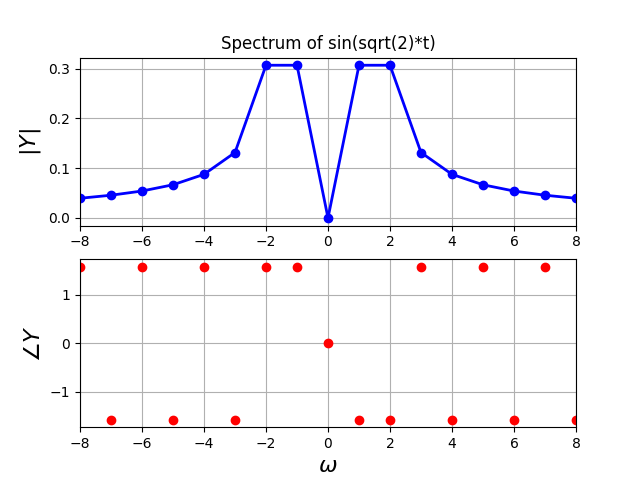
\includegraphics[scale=0.8]{Figure_1.png}
\end{figure}

This is because, the DFT is trying to analyse the 2$\pi$ periodic extension
of the function in the interval [-$\pi$, $\pi$] . This function, having discontinuities,
results in a slowly decaying frequency response and hence we do not obtain
shark peaks at the expected frequencies.

\subsection*{Windowing}
The fix for the above issue is to use windowing, we use the Hamming window function, the DFT after windowing shows significant improvement.

\begin{lstlisting}[language = Python]
Y, w = find_fft_np('sin',N=512,t_lim_1=-np.pi,t_lim_2=np.pi,windowing=True,x_limit=8,plot=True)
\end{lstlisting}
The following plot is obtained:
\begin{figure}[H]
     \centering
     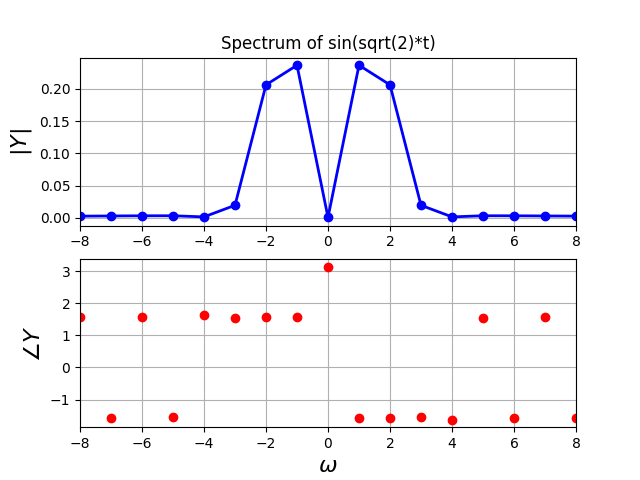
\includegraphics[scale=0.8]{Figure_2.png}
\end{figure}

The DFT is further improved by taking a larger time window.
\begin{lstlisting}[language = Python]
Y, w = find_fft_np('sin',N=512,t_lim_1=-4*np.pi,t_lim_2=4*np.pi,windowing=True,x_limit=4,plot=True)
\end{lstlisting}
The following plot is obtained:
\begin{figure}[H]
     \centering
     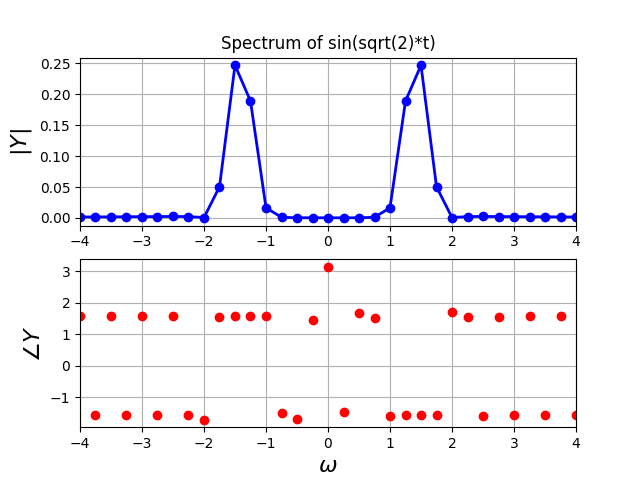
\includegraphics[scale=0.8]{Figure_3.png}
\end{figure}

\section{Question 2}
The spectrum of $\cos^3(\omega*t)$ without windowing for $\omega = 0.86$:
\begin{lstlisting}[language = Python]
Y, w = find_fft_np('cos3',N=512,t_lim_1=-4*np.pi,t_lim_2=4*np.pi,windowing=False)

\end{lstlisting}
The following plot is obtained:
\begin{figure}[H]
     \centering
     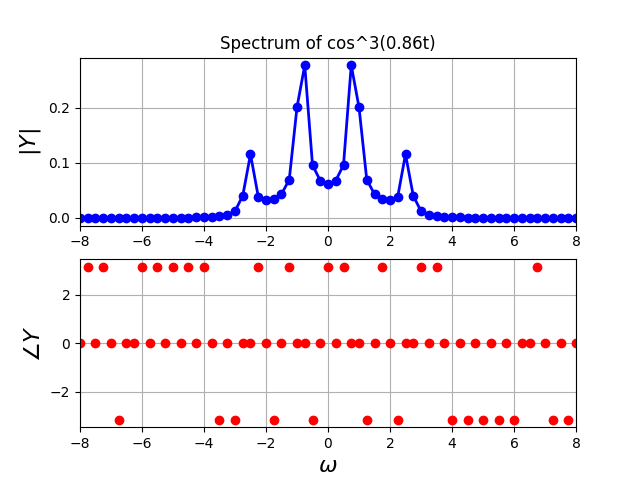
\includegraphics[scale=0.8]{Figure_4.png}
\end{figure}

The spectrum of $\cos^3(\omega*t)$ with windowing for $\omega = 0.86$:
\begin{lstlisting}[language = Python]
Y, w = find_fft_np('cos3',N=512,t_lim_1=-4*np.pi,t_lim_2=4*np.pi,windowing=True)

\end{lstlisting}
The following plot is obtained:
\begin{figure}[H]
     \centering
     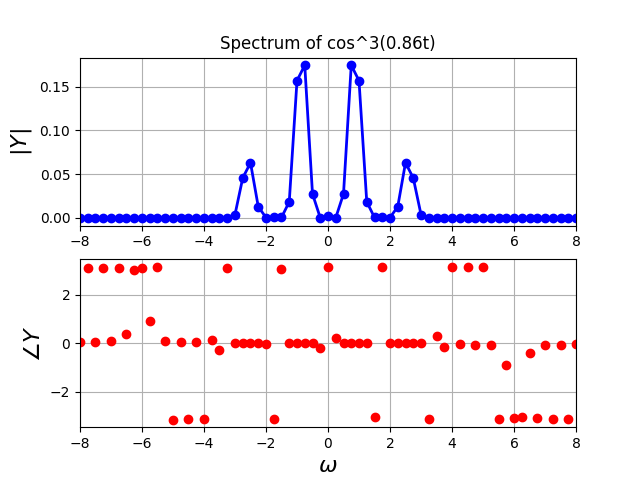
\includegraphics[scale=0.8]{Figure_5.png}
\end{figure}

\section{Question 3: Estimation of $\omega$ and $\delta$ using the DFT}
Given a 128 element vector known to contain $\cos(\omega_0*t+\delta)$ for arbitrary $\delta$ and $0.5 < \omega_0 < 1.5$ , we try to estimate the value of $\omega_0$ and $\delta$ using the DFT of the vector.

Due to the very low sampling rate, the resolution in the frequency domain is low, the following are the functions defined.

\begin{lstlisting}[language = Python]
def cos1(t, w0 = 1.5, delta = np.pi/2):
    return np.cos(w0*t+delta)
functions['cos1'] = cos1
get_title['cos1'] = 'Spectrum of cos(1.5*t+pi/2)'
def cos_withnoise(t, w0 = 1.5, delta = np.pi/2, A = 0.1):
    return np.cos(w0*t+delta)+A*np.random.randn(len(t))
functions['cos_withnoise'] = cos_withnoise
get_title['cos_withnoise'] = 'Spectrum of cos(1.5*t+pi/2) with white Gaussian noise'
\end{lstlisting}

The following plot is obtained for $\cos(1.5*t+\pi/2)$:
\begin{figure}[H]
     \centering
     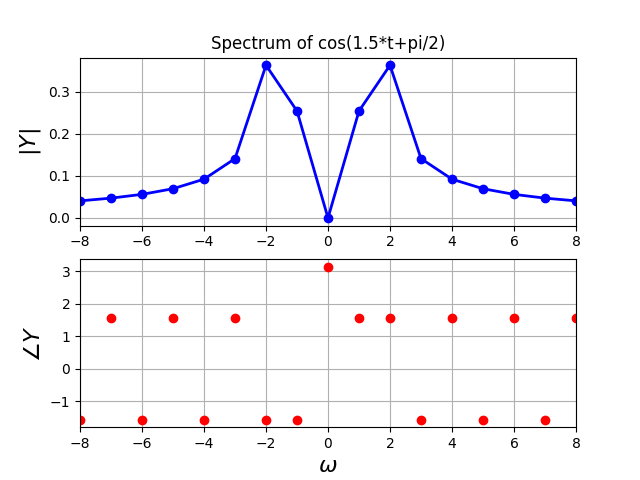
\includegraphics[scale=0.8]{Figure_6.png}
\end{figure}

As we see, the peaks are not accurately placed, and thus it is challenging to obtain a good estimate. By simply noticing that expectation value of $\omega_0$ over Y should produce results close to the true value, we experiment with our estimation method as:
\[\omega_{0,est} = \frac{\Sigma |Y|^p*w}{\Sigma|Y|^p}\]

The code for this is as follows:

\begin{lstlisting}[language = Python]
#Question 3
t = np.linspace(-np.pi,np.pi,128+1);t=t[:-1]

#Assuming w0 = 1.25 and delta = pi/2
y = functions['cos1'](t,1.5,np.pi/2)

dt = t[1]-t[0]
fmax = 1/dt
n = np.arange(128)
wnd = np.fft.fftshift(0.54+0.46*np.cos(2*np.pi*n/(128-1)))
y = y*wnd
y[0] = 0
y = np.fft.fftshift(y)
Y = np.fft.fftshift(np.fft.fft(y))/128
w = np.linspace(-np.pi*fmax,np.pi*fmax,128+1);w=w[:-1]
find_fft_np('cos1',N=128,t_lim_1=-np.pi,t_lim_2=np.pi,windowing=False)

ii = np.where(w>=0)
p = 1.7
w_cal = sum(abs(Y[ii])**p*w[ii])/sum(abs(Y[ii])**p)
i = abs(w-w_cal).argmin()
delta = np.angle(Y[i])
print("Calculated value of w0 without noise: ",w_cal)
print("Calculated value of delta without noise: ",delta)



\end{lstlisting}

On experimenting with different values of p, it was found that a value of
$p = 1.7$ gave good results in the given range of $\omega_0$.

For estimating $\delta$, we know that the DFT of a sinusoid must have two peaks at $\pm$ the natural frequency, thus, the phase is found by observing the phase at $\omega_0$ which is the peak value of the magnitude spectrum.

The results:
\begin{figure}[H]
     \centering
     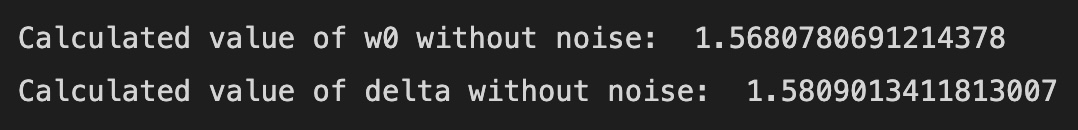
\includegraphics[scale=0.6]{Figure_10.png}
\end{figure}

\section{Question 4}
In the case of added gaussian noise, the parameter p used in frequency estimation has to be changed, while the phase estimation algorithm would still
work, considering the fact that the DFT of a gaussian is a gaussian in frequency, and for the given range of wo, the phase remains almost unaffected.
Through an exhaustive grid search (beyond the scope of this assignment), the parameter p = 2.4 gave good results
for this case. 

Plot:
\begin{figure}[H]
     \centering
     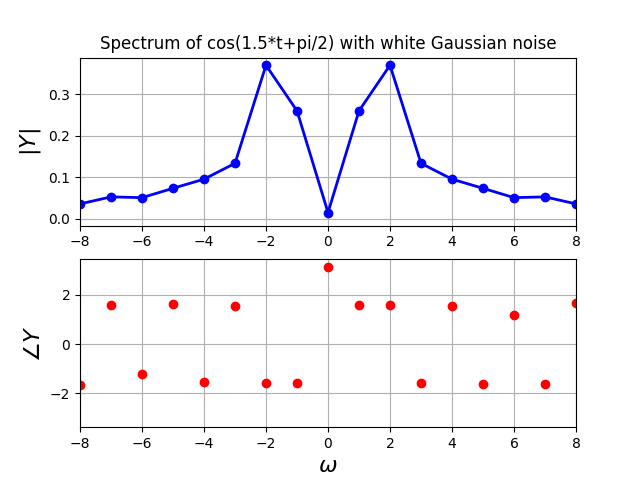
\includegraphics[scale=0.8]{Figure_7.png}
\end{figure}

The Results:
\begin{figure}[H]
     \centering
     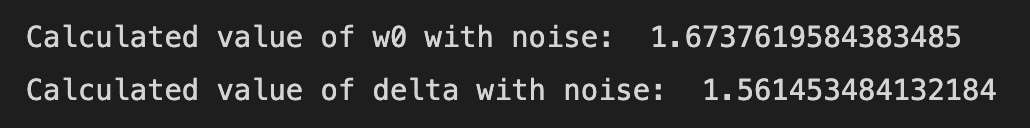
\includegraphics[scale=0.6]{Figure_11.png}
\end{figure}

\section{Question 5: DFT of a chirped signal}
The chirped signal is a signal of varying frequency, with frequency increasing
from 16 to 32 radians per second as we move from $-\pi$ to $\pi$.

\[chirp(t) = \cos(16(1.5+ t/(2*\pi))t)\]

\begin{lstlisting}[language = Python]
t = np.linspace(-np.pi,np.pi,1024+1);t=t[:-1]
chirp = functions['chirp'](t)
#plotting chirp function
plt.figure()
plt.plot(t,chirp)
plt.xlabel('t')
plt.ylabel('chirp')
plt.title('chirp function')
plt.grid(True)
plt.show()
find_fft_np('chirp', N=1024, t_lim_1=-np.pi, t_lim_2=np.pi,windowing=False, x_limit = 50)

\end{lstlisting}

The following plots are obtained:
\begin{figure}[H]
     \centering
     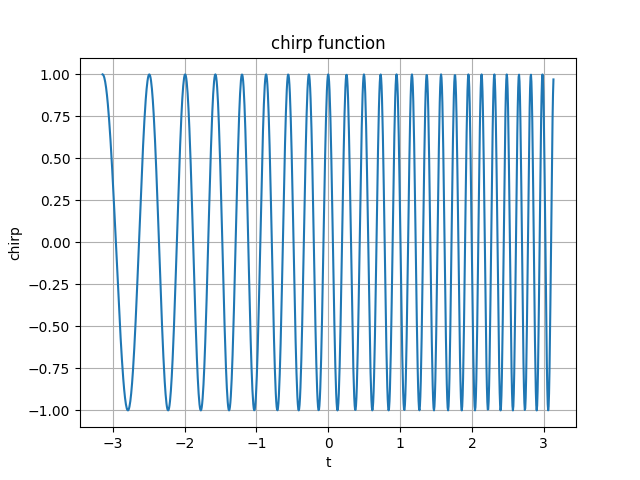
\includegraphics[scale=0.7]{Figure_12.png}
\end{figure}
\begin{figure}[H]
     \centering
     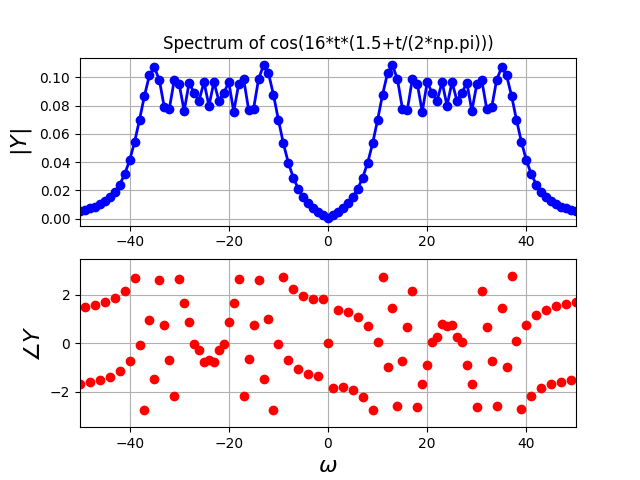
\includegraphics[scale=0.7]{Figure_8.png}
\end{figure}

On breaking the 1024 length vector into 16 pieces, each 64 samples wide,
we can analyse the DFT in how it evolves over time.

This is done by plotting a surface plot using the following snippet:

\begin{lstlisting}[language = Python]
t = np.linspace(-np.pi,np.pi,1024+1);t=t[:-1]
#split t into 16 arrays of length 64
t_split = np.array_split(t,16)
Y = []
for t in t_split:
    Y.append(find_fft_np('chirp', N=64, t_lim_1=t[0], t_lim_2=t[-1], windowing=False, x_limit = 50, plot = False)[0])
Y = np.array(Y)

t1 = np.linspace(-np.pi,np.pi,16+1);t1=t1[:-1]
dt = t[1] - t[0]
fmax = 1/dt
w = np.linspace(-np.pi*fmax,np.pi*fmax,64+1);w=w[:-1]
Y1 = Y.copy()
indices = np.where(w>150)
Y1[:,indices] = 0

#plotting surface plot
import mpl_toolkits.mplot3d.axes3d as p3
fig = plt.figure()
ax = p3.Axes3D(fig)
t1, w = np.meshgrid(t1,w)
ax.plot_surface(t1, w, abs(Y1.T), rstride = 1, cstride = 1, cmap=plt.cm.viridis)
ax.set_xlabel('t')
ax.set_ylabel('w')
ax.set_zlabel('Y')
plt.show()

\end{lstlisting}

The plot obtained is as follows:

\begin{figure}[H]
     \centering
     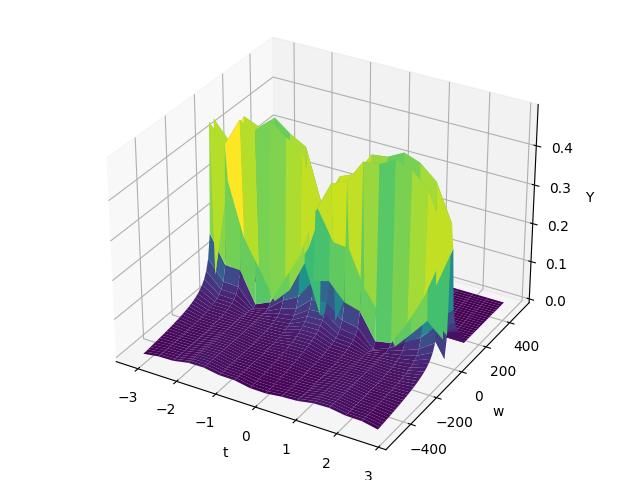
\includegraphics[scale=0.6]{Figure_9.png}
\end{figure}
We observe that the peak frequency increases with time.

\section{Conclusion}
The DFT was obtained using a 2$\pi$ periodic extension of the signal, which was found to be not very accurate. The
spectrum was rectified by the using a windowing technique, by employing the
Hamming window. \\Given a vector of cosine values in the a time interval, the
frequency and phase were estimated from the DFT spectrum, by using the
expectation value of the frequency. \\The DFT of a chirped signal was analysed and its time-frequency plot showed the gradual variation of peak frequency of the spectrum with time.















\end{document}